\documentclass{article}
\usepackage{fontspec,tikz,graphicx}
\setmainfont{Times New Roman}
\usepackage[a3paper,margin=1cm]{geometry}
\pagestyle{empty}
\begin{document}
\noindent\resizebox{\textwidth}{!}{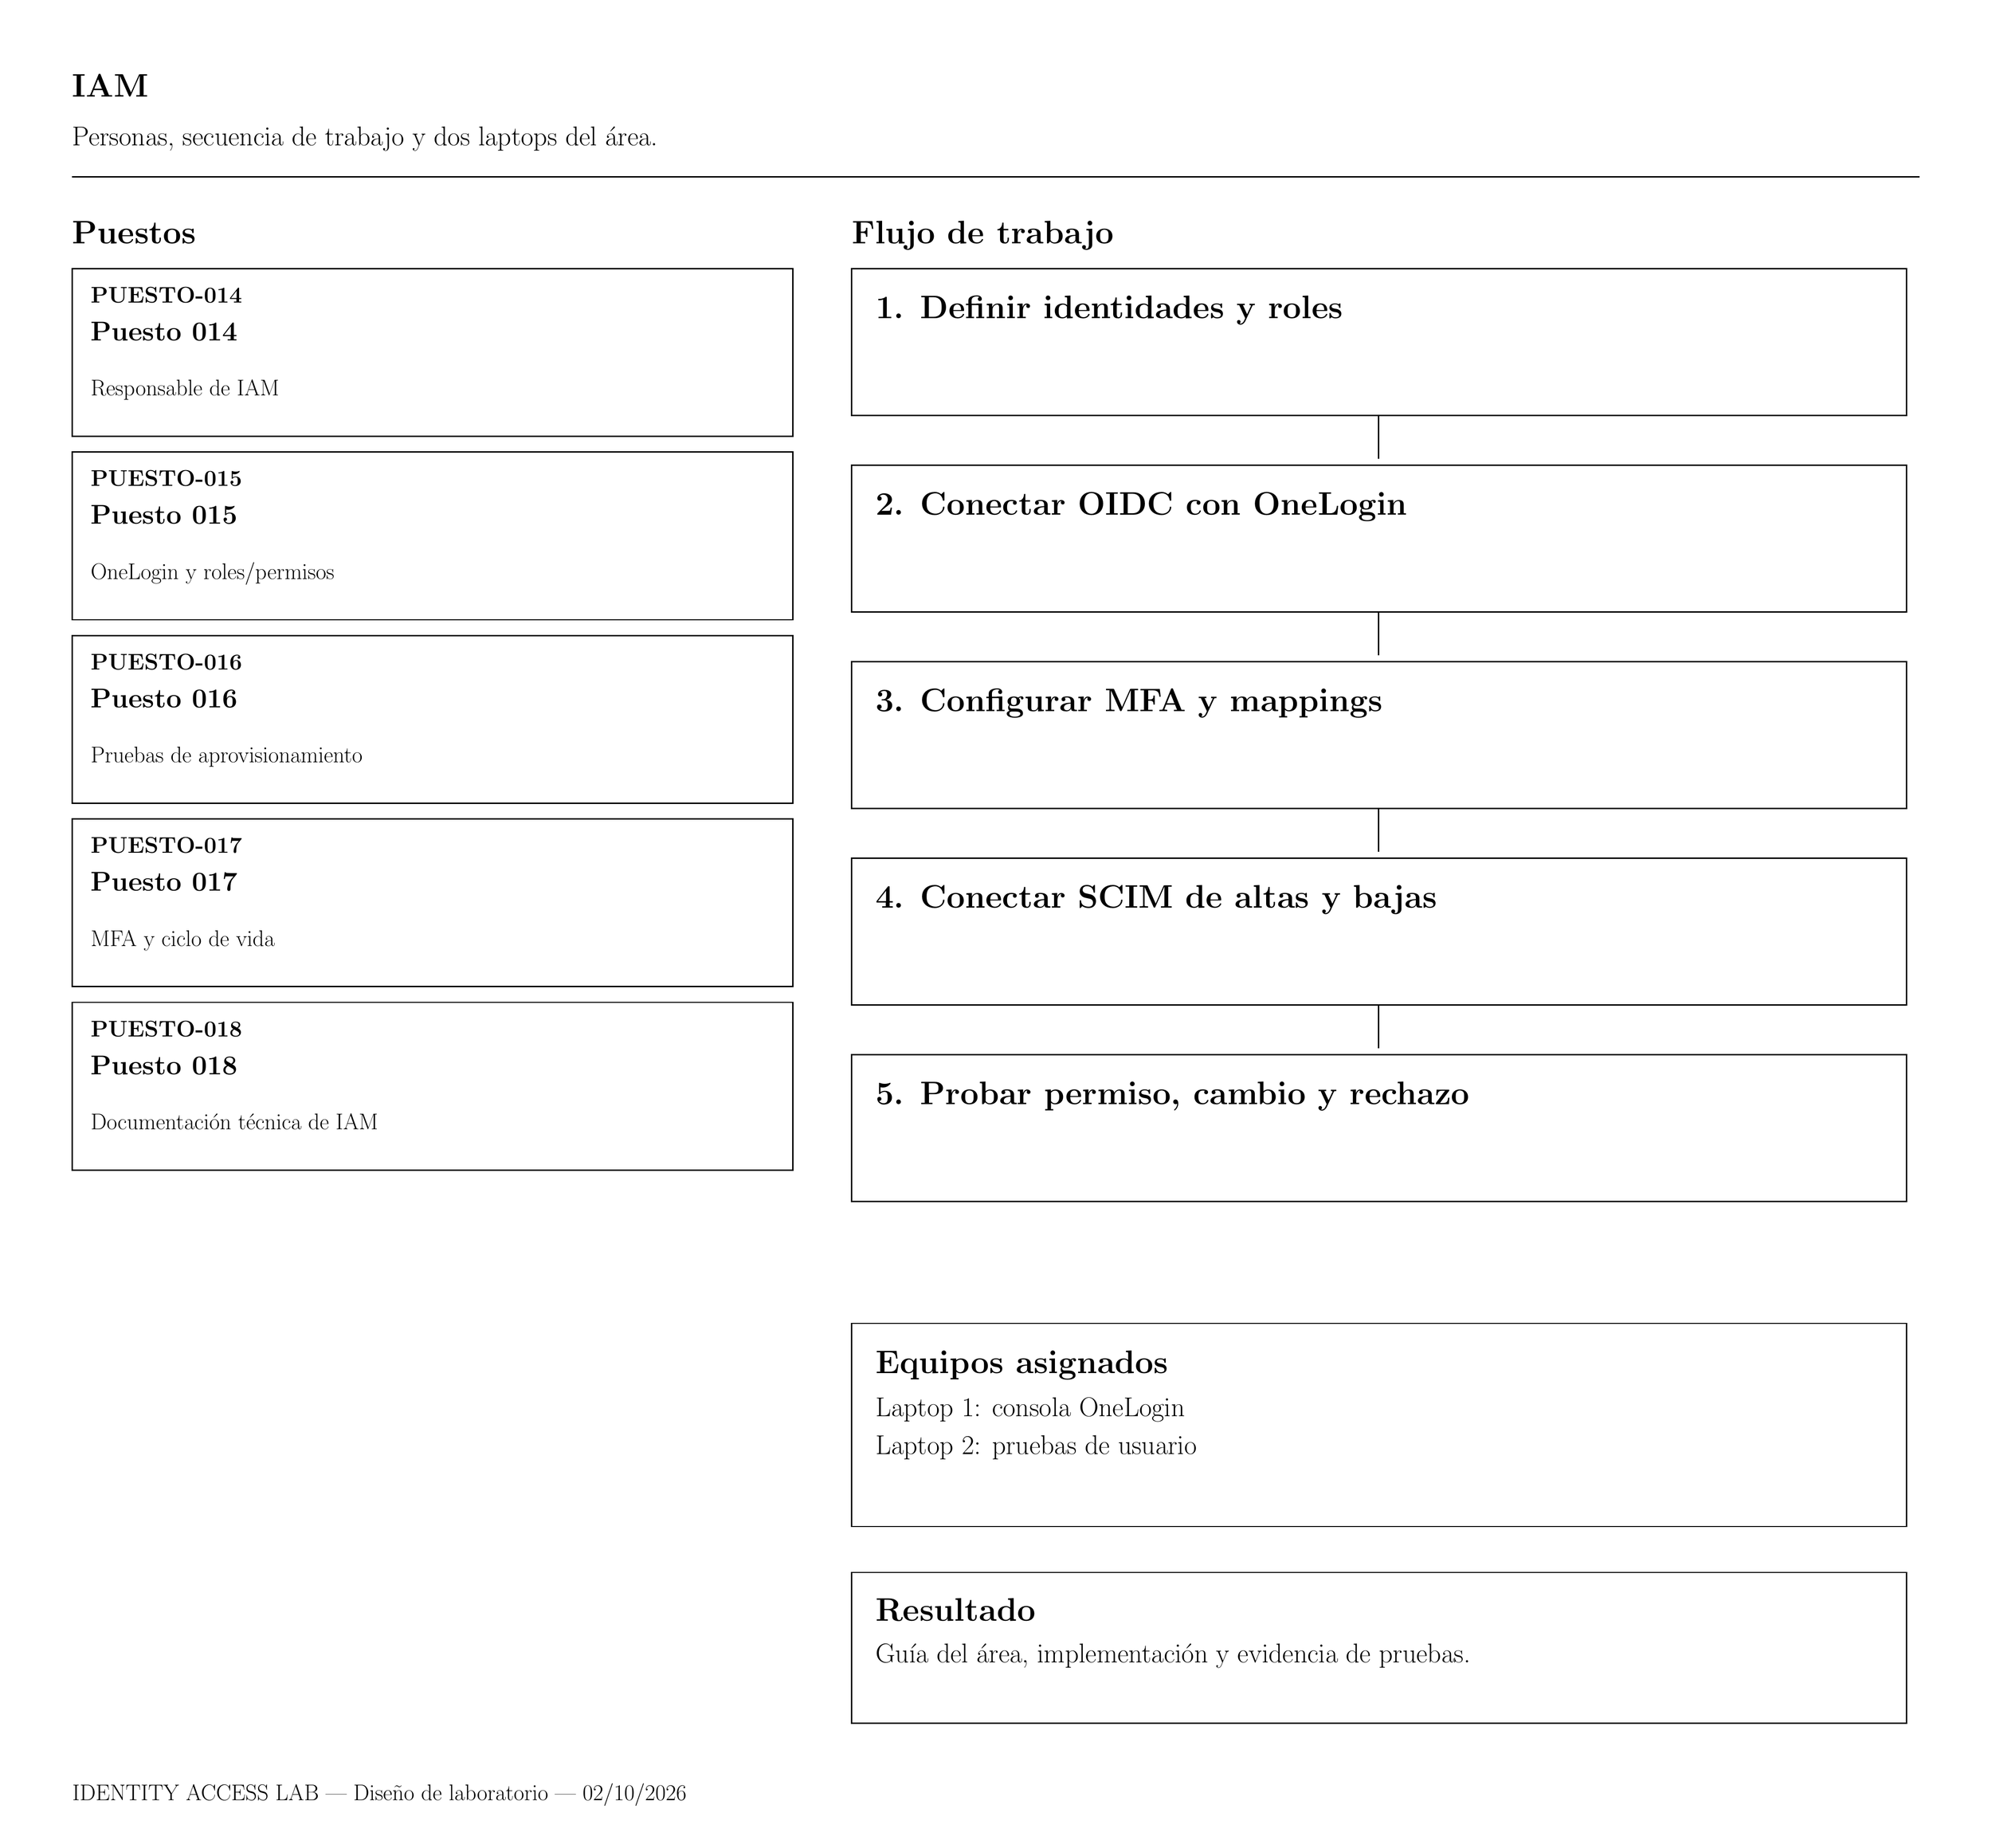
\begin{tikzpicture}[x=1pt,y=-1pt]
\path[use as bounding box] (0,0) rectangle (1500.0,1390.0);
\node[anchor=base west,inner sep=0pt,font=\fontsize{34.0}{40.8}\selectfont \bfseries ] at (45,64) {IAM};
\node[anchor=base west,inner sep=0pt,font=\fontsize{21.0}{25.2}\selectfont ] at (45,101) {Personas, secuencia de trabajo y dos laptops del área.};
\draw[line width=1pt] (45,125) -- (1455,125);
\node[anchor=base west,inner sep=0pt,font=\fontsize{25.0}{30.0}\selectfont \bfseries ] at (45,176) {Puestos};
\node[anchor=base west,inner sep=0pt,font=\fontsize{25.0}{30.0}\selectfont \bfseries ] at (640,176) {Flujo de trabajo};
\draw[line width=1pt] (45.0,195.0) rectangle (595.0,323.0);
\node[anchor=base west,inner sep=0pt,font=\fontsize{18.0}{21.599999999999998}\selectfont \bfseries ] at (59,221) {PUESTO-014};
\node[anchor=base west,inner sep=0pt,font=\fontsize{20.0}{24.0}\selectfont \bfseries ] at (59,250) {Puesto 014};
\node[anchor=base west,inner sep=0pt,font=\fontsize{19.0}{22.8}\selectfont ] at (59,292) {Responsable de IAM};
\draw[line width=1pt] (45.0,335.0) rectangle (595.0,463.0);
\node[anchor=base west,inner sep=0pt,font=\fontsize{18.0}{21.599999999999998}\selectfont \bfseries ] at (59,361) {PUESTO-015};
\node[anchor=base west,inner sep=0pt,font=\fontsize{20.0}{24.0}\selectfont \bfseries ] at (59,390) {Puesto 015};
\node[anchor=base west,inner sep=0pt,font=\fontsize{19.0}{22.8}\selectfont ] at (59,432) {OneLogin y roles/permisos};
\draw[line width=1pt] (45.0,475.0) rectangle (595.0,603.0);
\node[anchor=base west,inner sep=0pt,font=\fontsize{18.0}{21.599999999999998}\selectfont \bfseries ] at (59,501) {PUESTO-016};
\node[anchor=base west,inner sep=0pt,font=\fontsize{20.0}{24.0}\selectfont \bfseries ] at (59,530) {Puesto 016};
\node[anchor=base west,inner sep=0pt,font=\fontsize{19.0}{22.8}\selectfont ] at (59,572) {Pruebas de aprovisionamiento};
\draw[line width=1pt] (45.0,615.0) rectangle (595.0,743.0);
\node[anchor=base west,inner sep=0pt,font=\fontsize{18.0}{21.599999999999998}\selectfont \bfseries ] at (59,641) {PUESTO-017};
\node[anchor=base west,inner sep=0pt,font=\fontsize{20.0}{24.0}\selectfont \bfseries ] at (59,670) {Puesto 017};
\node[anchor=base west,inner sep=0pt,font=\fontsize{19.0}{22.8}\selectfont ] at (59,712) {MFA y ciclo de vida};
\draw[line width=1pt] (45.0,755.0) rectangle (595.0,883.0);
\node[anchor=base west,inner sep=0pt,font=\fontsize{18.0}{21.599999999999998}\selectfont \bfseries ] at (59,781) {PUESTO-018};
\node[anchor=base west,inner sep=0pt,font=\fontsize{20.0}{24.0}\selectfont \bfseries ] at (59,810) {Puesto 018};
\node[anchor=base west,inner sep=0pt,font=\fontsize{19.0}{22.8}\selectfont ] at (59,852) {Documentación técnica de IAM};
\draw[line width=1pt] (640.0,195.0) rectangle (1445.0,307.0);
\node[anchor=base west,inner sep=0pt,font=\fontsize{24.0}{28.799999999999997}\selectfont \bfseries ] at (658,233) {1. Definir identidades y roles};
\draw[line width=1pt] (1042,307) -- (1042,340);
\draw[line width=1pt] (640.0,345.0) rectangle (1445.0,457.0);
\node[anchor=base west,inner sep=0pt,font=\fontsize{24.0}{28.799999999999997}\selectfont \bfseries ] at (658,383) {2. Conectar OIDC con OneLogin};
\draw[line width=1pt] (1042,457) -- (1042,490);
\draw[line width=1pt] (640.0,495.0) rectangle (1445.0,607.0);
\node[anchor=base west,inner sep=0pt,font=\fontsize{24.0}{28.799999999999997}\selectfont \bfseries ] at (658,533) {3. Configurar MFA y mappings};
\draw[line width=1pt] (1042,607) -- (1042,640);
\draw[line width=1pt] (640.0,645.0) rectangle (1445.0,757.0);
\node[anchor=base west,inner sep=0pt,font=\fontsize{24.0}{28.799999999999997}\selectfont \bfseries ] at (658,683) {4. Conectar SCIM de altas y bajas};
\draw[line width=1pt] (1042,757) -- (1042,790);
\draw[line width=1pt] (640.0,795.0) rectangle (1445.0,907.0);
\node[anchor=base west,inner sep=0pt,font=\fontsize{24.0}{28.799999999999997}\selectfont \bfseries ] at (658,833) {5. Probar permiso, cambio y rechazo};
\draw[line width=1pt] (640.0,1000.0) rectangle (1445.0,1155.0);
\node[anchor=base west,inner sep=0pt,font=\fontsize{24.0}{28.799999999999997}\selectfont \bfseries ] at (658,1038) {Equipos asignados};
\node[anchor=base west,inner sep=0pt,font=\fontsize{22.0}{26.4}\selectfont ] at (658,1071) {Laptop 1: consola OneLogin};
\node[anchor=base west,inner sep=0pt,font=\fontsize{22.0}{26.4}\selectfont ] at (658,1100) {Laptop 2: pruebas de usuario};
\draw[line width=1pt] (640.0,1190.0) rectangle (1445.0,1305.0);
\node[anchor=base west,inner sep=0pt,font=\fontsize{23.0}{27.599999999999998}\selectfont \bfseries ] at (658,1227) {Resultado};
\node[anchor=base west,inner sep=0pt,font=\fontsize{21.0}{25.2}\selectfont ] at (658,1259) {Guía del área, implementación y evidencia de pruebas.};
\node[anchor=base west,inner sep=0pt,font=\fontsize{18.0}{21.599999999999998}\selectfont ] at (45,1364) {IDENTITY ACCESS LAB | Diseño de laboratorio | 02/10/2026};
\end{tikzpicture}}
\end{document}
